\chapter{FPGA Implementation}\label{chap:FPGA_Implementation}
This chapter is devoted to discussing how to implement a Chipyard-generated processor design on a \textbf{local} \gls{fpga} for quicker testing and general use.
Throughout the research project this manual was originally completed in, the Arty \gls{fpga} was used.
An image of the Arty board can be seen in \Cref{fig:Arty_FPGA}.
The Arty board is built using a Xilinx \gls{fpga} module and then Arty creates a board surrounding the particular chip.

\begin{figure}[h!tbp]
  \centering
  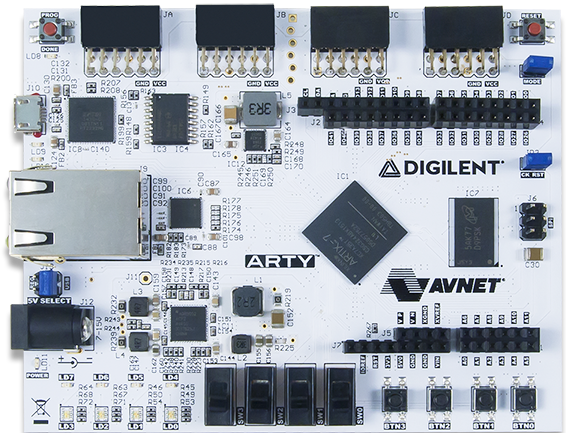
\includegraphics[scale=0.35]{./Arty_FPGA.png}
  \caption{Arty \Gls{fpga}}
  \label{fig:Arty_FPGA}
\end{figure}

\section{About}\label{sec:About}
The Chipyard Framework contains initial support for \gls{fpga} development and simulation of \gls{soc} designs.
At the moment this support is very limited, and is in active development.
As of \today, the best support for \Gls{fpga} Development for the Arty 35T \Gls{fpga} comes from a branch of Chipyard called \href{https://github.com/ucb-bar/chipyard/tree/arty-spi-flash}{arty-spi-flash}.
This branch fixes the \gls{uart} implementation and enables the \gls{spi} flash storage on the Arty \Gls{fpga} to allow users to store programs.

\section{Prerequisites}\label{sec:Prerequisites}
To assist with the proper setup, we approached the \Gls{fpga} implementation of an \Gls{soc} by following the \citetitle{FreedomDevGuide}~\cite{FreedomDevGuide}.
This outlined many of the steps we would eventually need to take, starting with purchasing an \href{https://www.digikey.com/en/products/detail/olimex-ltd/ARM-USB-TINY-H/3471388}{Olimex JTAG Debugger}~\cite{OlimexJTAG}.
Once the final image is flashed to the \Gls{fpga}, the debugger will allow the user to upload C programs and execute them on the RISC-V processor.
Without the \gls{jtag} Debugger, we were unable to upload programs to the \Gls{fpga}, so this is a necessity.

\begin{figure}[h!tbp]
  \centering
  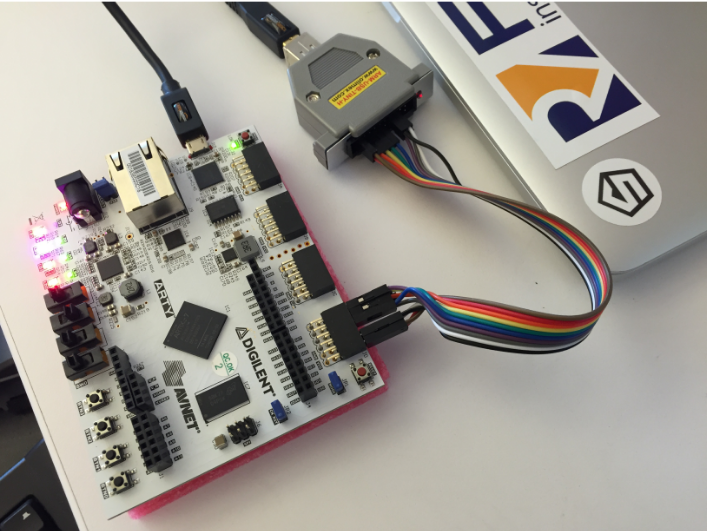
\includegraphics[width=0.7\linewidth]{./OlimexSetup.png}
  \caption{Olimex Debugger Setup~\cite[p.~5]{FreedomDevGuide}}
  \label{fig:olimexsetup}
\end{figure}

\begin{figure}
	\centering
	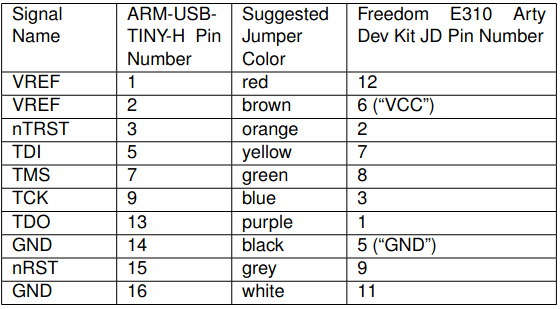
\includegraphics[width=0.7\linewidth]{./JTAG_connections.png}
	\caption{Olimex Debugger Pin Connections~\cite[p.~4]{FreedomDevGuide}}
	\label{fig:olimexpins}
\end{figure}

\section{Customizing an FPGA Image}\label{sec:Customizing}
In Chipyard, the directory used for all \Gls{fpga} prototyping functionality is \file{chipyard/fpga}, located in the root directory.
Inside this directory there are several important files.


\subsection{Configuration Directory}\label{sec:Customizing_FPGA-Config_Directory}
The configuration directory for the Arty \Gls{fpga} is located under \file{chipyard/fpga/src/main/scala/arty/}.
This directory includes several useful files, including \file{Configs.scala}, \file{HarnessBinders.scala}, \file{IOBinders.scala}, and \file{TestHarness.scala}.

\subsubsection{\file{Configs.scala}}\label{sec:Customizing_FPGA-Configs.scala}
This file is where custom Chipyard SoC configurations are stored and utilized for \Gls{fpga} prototyping.
There are several custom configuration parameters for the Arty \Gls{fpga} in this file.
The default configuration utilized to make an image for the Arty board is labeled as \texttt{TinyRocketArtyConfig}, which then utilized the custom parameters defined for \texttt{WithArtyTweaks} and \texttt{WithDefaultPeripherals} in the same file.
The addresses specified in the \texttt{WithDefaultParameters} configurations alter how the memory mapped peripherals for the Arty \Gls{fpga} will be connected.

\subsubsection{\file{HarnessBinders.scala}}\label{sec:Customizing_FPGA-HarnessBinders.scala}
This file is where custom "harness binders"
\footnote{Harness Binders are utilized by Chipyard to connect the name of pins in HDL to the pins in the \texttt{TestHarness} Verilog model. To connect to the physical pins of the FPGA board, IOBinders will map the TestHarness pins to the physical pins of the FPGA.}
 for the Arty \Gls{fpga} are defined.
These harness binders utilize pins specified in the master \texttt{ArtyShell} pin definitions file for the Arty board (provided by Digilent for use in Xilinx Vivado).
This file is located at \file{chipyard/fpga/fpga-shells/src/main/scala/shell/xilinx/ArtyShell.scala}.
The pin mappings in this file are the same mappings that would be utilized when interfacing with the Arty board when designing in Xilinx Vivado.
Harness binders in this file are provided for the \Gls{jtag} interface, \Gls{spi} flash, and the \Gls{uart}  connector.
These three connections are critical to the \Gls{fpga} design, and to ensuring that programs can be successfully uploaded and run on the \Gls{fpga}.
It is important to note that the harness binders connects to the \texttt{TestHarness}, and not the physical IO~\cite{Chipyard_IO}.
This was done such that separation could be created between the simulated and physical designs.
To connect to the physical IO pins, IOBinders are also needed.

\subsubsection{\file{IOBinders.scala}}\label{sec:Customizing_FPGA-IOBinders.scala}
This file is where the physical IO pins are connected to the harness binders defined previously.
In this file are custom configurations for the \Gls{spi} flash and \Gls{jtag} connectors that will be utilized in the default design.
In the future, additional IOBinders for other peripherals on the Arty \Gls{fpga} should be implemented.

\subsubsection{\file{TestHarness.scala}}\label{sec:Customizing_FPGA-TestHarness.scala}
This file is where miscellaneous connections are made between pins, global clock and reset variable are defined, and the Harness Binders are actually applied to the \Gls{soc} design.
No modification to this file should be needed in order to implement new peripheral devices in the future.

% \subsection{generated-src Directory}\label{sec:Customizing_FPGA-Generated-src_Directory}

The generated-src directory is the directory in which all files created from compiling the \Gls{soc} design and \Gls{fpga} image will be stored.
This means that the memory map, \Gls{fpga} bitstream, and other important files will be stored in this directory.
This directory can be found at \file{chipyard/fpga/generated-src}.
This directory will not be created until a \Gls{fpga} design run is initiated.

\subsection{Makefile}\label{sec:Customizing_FPGA-Makefile}
Inside the Makefile is where you are able to define a custom subproject as shown in \Cref{subsec:Makefile_SUB_PROJECT} and \Cref{subsec:Building_Each_Subproject}.
This allows users to control what files are compiled and generated for the \Gls{fpga} image.
This is highly recommended as it simplifies the workflow for repeated compilation attempts.

\section{Generating the FPGA Image}\label{sec:Generating_FPGA_Image}

\subsection{Syntax}\label{sec:Generating_FPGA_Image-Syntax}
Much like generating a verilog simulation, there are many options when it comes to generating an FPGA image in Chipyard.
The complete syntax is as follows:~\cite{Chipyard_Prototyping}

\begin{listing}[h!tbp]
  \begin{bashsource}
    make SBT_PROJECT=... MODEL=... VLOG_MODEL=... MODEL_PACKAGE=... CONFIG=... CONFIG_PACKAGE=... GENERATOR_PACKAGE=... TB=... TOP=... BOARD=... FPGA_BRAND=... [-j[N]] bitstream
  \end{bashsource}
  \caption{Command to generate \Gls{fpga} image using long format}
  \label{lst:extended_fpga_cmd}
\end{listing}

The condensed syntax, as implemented in \cref{sec:Customizing_FPGA-Makefile} is as follows:

\begin{listing}[h!tbp]
  \begin{bashsource}
    make SUB_PROJECT=<sub_project> [-j[N]] bitstream
  \end{bashsource}
  \caption{Command to generate \Gls{fpga} image using subproject.}
  \label{lst:condensed_fpga_cmd}
\end{listing}

\begin{listing}[h!tbp]
	\begin{bashsource}
		ifeq ($(SUB_PROJECT),artyCustom) # Customize SUB_PROJECT name to artyCustom
			SBT_PROJECT       ?= fpga_platforms
			MODEL             ?= ArtyFPGATestHarness #Still utilize Arty Test Harness
			VLOG_MODEL        ?= ArtyFPGATestHarness 
			MODEL_PACKAGE     ?= chipyard.fpga.arty
			CONFIG            ?= ArtyCustomConfig #Change SoC configuration to build
			CONFIG_PACKAGE    ?= chipyard.fpga.arty #Package where custom config can be found
			GENERATOR_PACKAGE ?= chipyard 
			TB                ?= none # unused
			TOP               ?= ChipTop
			BOARD             ?= arty
			FPGA_BRAND        ?= xilinx
		endif
	\end{bashsource} 
	\caption{Example of sub project variables customization}
	\label{lst:$makefile_subproject_example}
\end{listing}

It is highly recommended to make use of the \texttt{-jN} flag to allow multi-threading and speed up generation.
Without multi-threading the process of generating an image can take multiple hours.

When generating the default Arty image, we noticed that the script would produce an error about \texttt{Failed to meet timing by \$timing\_slack}.
However, we found that the image still appears to run correctly, so further investigation is needed into why this error occurs.

Upon successful generation, the bitstream file will be saved to \\ \file{chipyard/fpga/generated-src/<long\_project\_name>/obj/<ConfigName>.bit}.

The branch of chipyard with the best functionality for the Arty board is currently the \texttt{arty-spi-flash} branch, so use of this branch is recommended.

\subsection{Creating MCS File}\label{sec:Creating_MCS_file}
After generating a bitstream file, one should utilize Xilinx Vivado to create a \gls{mcs} file in order to save the design to the SPI flash on the Arty board.
This will allow the design to be automatically reloaded onto the Arty board after power is disconnected.

To begin, open Xilinx Vivado, and enter the \texttt{Hardware Manager} (shown in \Cref{fig:Vivado_HW_Manager}).
Under the \texttt{Tools} dropdown, select \texttt{Generate Memory Configuration File}.
\begin{figure}[h!tbp]
  \centering
  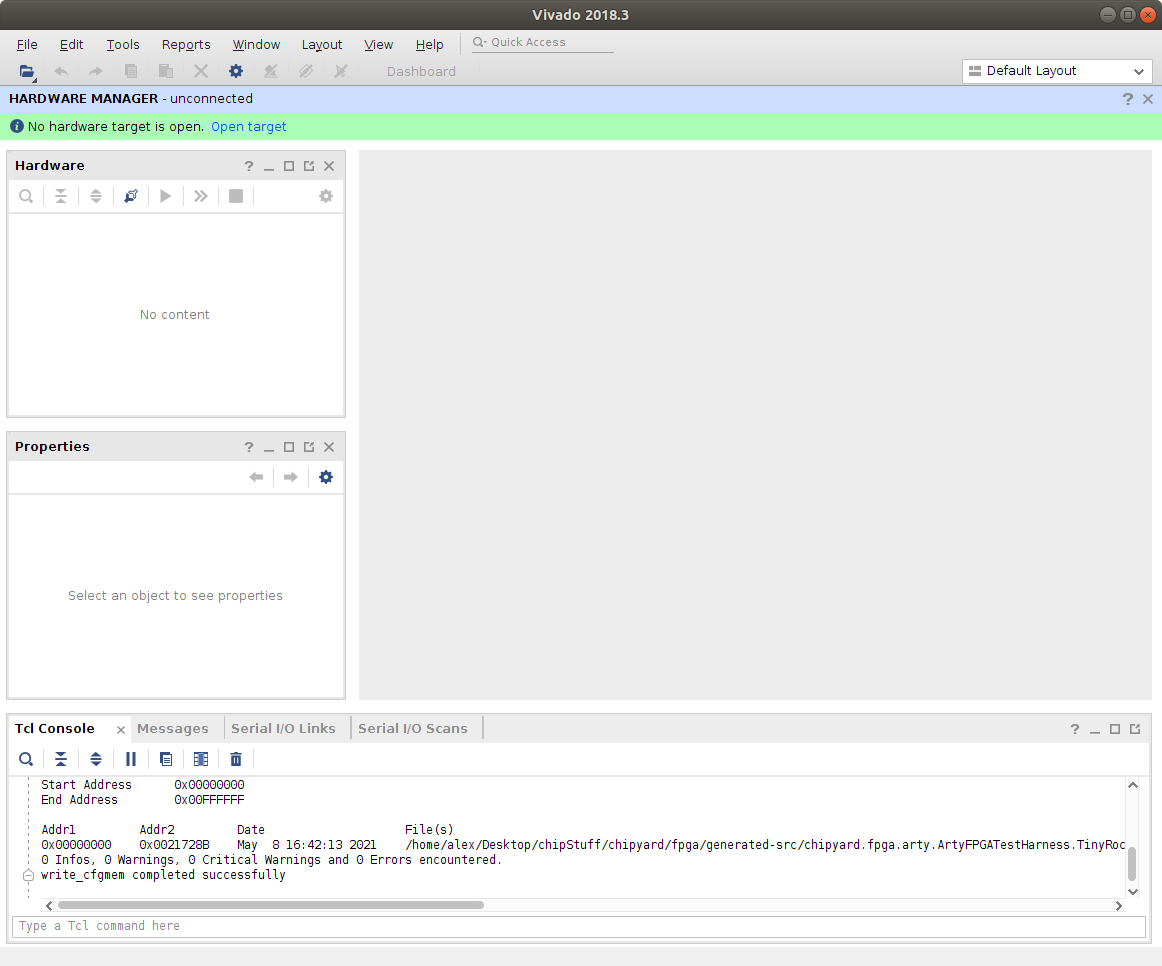
\includegraphics[scale=0.20]{./Vivado_HW_Manager.png}
  \caption{Vivado Hardware Manager Window}
  \label{fig:Vivado_HW_Manager}
\end{figure}

Inside this wizard (shown in \Cref{fig:Vivado_MCS_Window}), there are several options that must be filled.
\begin{description}
\item[Memory Part] Select the memory part present on your specific \Gls{fpga} board.
  For the Arty board we used, this was the \texttt{s25fl128sxxxxxx0-spi-x1\_x2\_x4} device.
\item[Filename] Specify a new output location and name for the MCS file that will be generated.
\item[Interface] Specify \Gls{spi}x4 for the Arty board. Other options include a x1 or x2 wide \Gls{spi} interface.
\item[Bitfile] Select the bitstream file generated previously by Chipyard.
\item[Datafile] In theory, this should allow one to upload a .hex or .elf program file to be run by the Arty board, however in our experience we had better success when uploaded using the \Gls{jtag} debugger after flashing the \Gls{fpga}.
\end{description}

\begin{figure}[h!tbp]
  \centering
  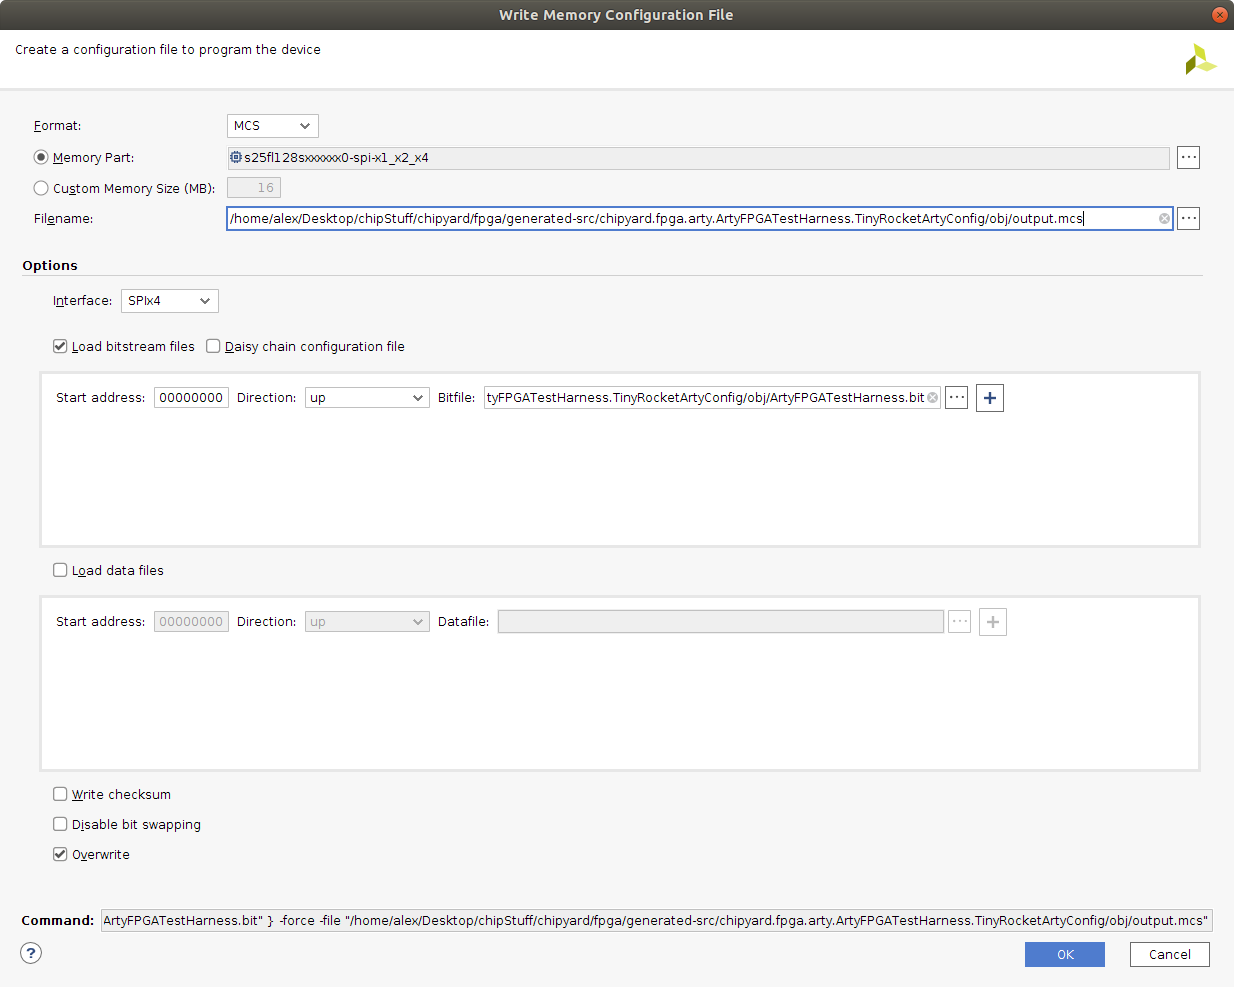
\includegraphics[scale=0.20]{./MCS_Generation_Window.png}
  \caption{Vivado MCS Generation Window}
  \label{fig:Vivado_MCS_Window}
\end{figure}

\section{Using the FPGA Image}\label{sec:Using_FPGA_Image}
\subsection{Flashing the Image}\label{sec:Flash_FPGA_Image}
In order to flash the MCS file generated in \Cref{sec:Creating_MCS_file}, first open Vivado Hardware Manager (\Cref{fig:Vivado_HW_Manager}) and connect the Arty board via USB.
Inside Hardware Manager, click the \texttt{Open target prompt} and select \texttt{Auto Connect} at the top of the window to connect to the Arty board.
In the Hardware section of the window, the Arty board will now be shown as \texttt{xc7a35t\_0} (shown in \Cref{fig:Vivado_HW_connected}).

\begin{figure}[h!tbp]
  \centering
  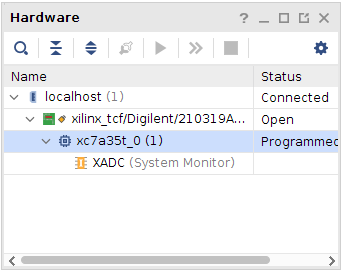
\includegraphics[scale=0.5]{./arty_connected_window.png}
  \caption{Hardware section of Vivado Hardware Manager}
  \label{fig:Vivado_HW_connected}
\end{figure}

Next, right-click on \texttt{xc7a35t\_0}, select \texttt{Add Configuration Memory Device}, and navigate to the same memory configuration device selected previously (\Cref{fig:add_config_mem}).
After clicking \texttt{OK}, you will be prompted to program the configuration memory device (\Cref{fig:prog_config_mem}).
In this prompt, select the \Gls{mcs} file generated previously.
After selecting \texttt{OK}, flashing of the image will commence.
At this point, if the wrong memory part was selected, you will receive an error message depicting the correct memory part.
If this occurs, repeat creating the \Gls{mcs} file (\Cref{sec:Creating_MCS_file}), adding the memory configuration device, and try again.

\begin{figure}[h!tbp]
  \centering
  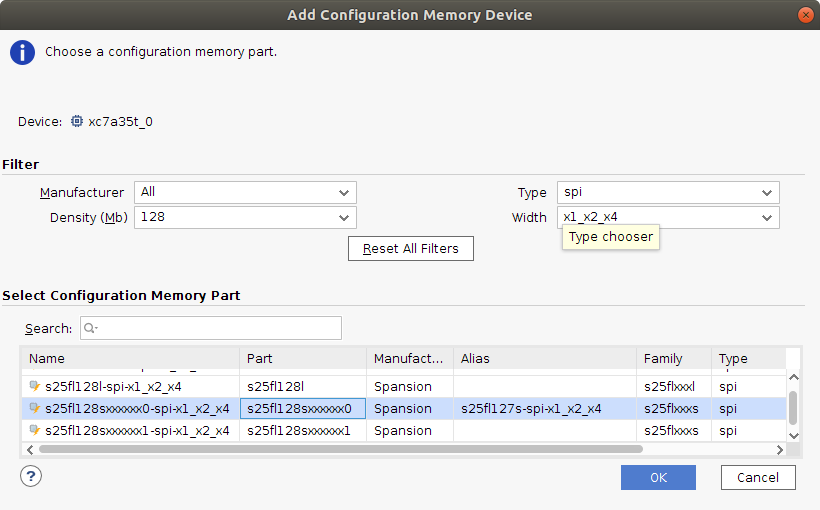
\includegraphics[scale=0.35]{./add_config_mem.png}
  \caption{Add Configuration Memory Device}
  \label{fig:add_config_mem}
\end{figure}

\begin{figure}[h!tbp]
  \centering
  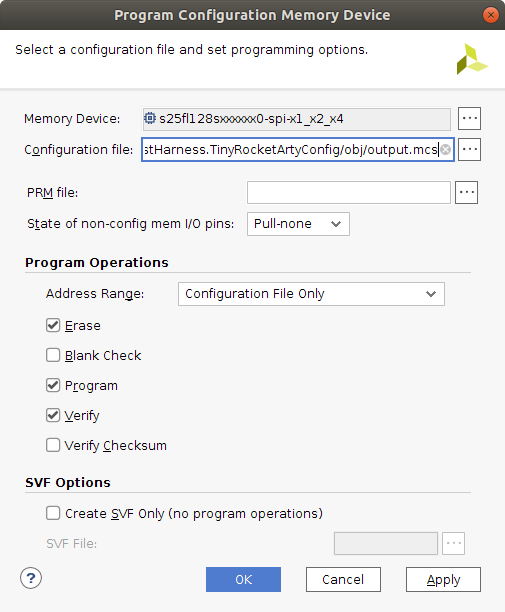
\includegraphics[scale=0.35]{./prog_config_mem.png}
  \caption{Program Configuration Memory Device}
  \label{fig:prog_config_mem}
\end{figure}

After the flashing of the MCS file, ensure that jumper JP1 is shorted so that the FPGA boots from the SPI flash, and press the \texttt{PROG} button on the Arty board.
The \texttt{DONE} LED on the Arty board should be lit, indicating that flashing the FPGA image was a success.
We can now proceed to compile and upload C programs to the \Gls{fpga}.

\subsection{Compiling Programs}\label{sec:Compiling_Programs}
In order to compile programs for the Arty board, we utilized the Freedom E SDK (Mentioned in \Cref{sec:Freedom_E_SDK}) project provided by SiFive~\cite{freedomESDK}.
To correctly configure the Freedom E SDK for the Chipyard Arty implementation, we must first specify the \Gls{jtag} debugger that will be used in this project.
This can be done in the file \file{/freedom-e-sdk/bsp/freedom-e310-arty/openocd.cfg}.
In this file, edit line 9 to \texttt{set protocol jtag} and line 14 to \texttt{set connection probe}.
These settings will allow the Freedom E SDK to utilize the Olimex debugger purchased for this project.

Documentation for the Freedom E SDK can be found at the \href{https://sifive.github.io/freedom-metal-docs/}{Freedom Metal Library Github page}.
It is important to note that much of the functionality regarding physical features (GPIO, Buttons, LEDs, etc.) are currently not functional on the Chipyard SoC implementation for the Arty.
Additionally, we found that some functionality in the Metal library was buggy. 
For example, sending output to the serial terminal did not work when using \mintinline{C}{printf()}, but did work when utilizing \mintinline{C}{putc()}.
In the future, compatibility and functionality should be improved for this C library.

In the Freedom E SDK, default and custom projects are defined in the directory \file{/freedom-e-sdk/software/}.
To compile a project for the Arty board, run the following command:

\begin{listing}[h!tbp]
  \begin{bashsource}
    make TARGET=freedom-e310-arty PROGRAM=<program> CONFIGURATION=debug software
  \end{bashsource}
  \caption{Command used to compile a program for the Arty board in the Freedom E SDK}
  \label{lst:compile_in_sdk}
\end{listing}

\subsection{Uploading Programs to the FPGA}\label{sec:Upload_Programs_to_Flashed_FPGA}
Before running a program on the Arty board, it is important to start a serial connection to the Arty board, so that you can view the serial output from the Arty board.
Other documentation has declared that the design should output to UART at a baud rate of 115200, however we have found that the correct baud rate is 57600.
The serial terminal we utilized for this project is CuteCom~\cite{CuteCom}, due to its ease of adjusting settings and graphical interface, although other options include GNU Screen, minicom, PuTTY, etc.

To load a default or custom project onto the Arty board, use the following syntax:

\begin{listing}[h!tbp]
  \begin{bashsource}
    make TARGET=freedom-e310-arty PROGRAM=<program> CONFIGURATION=debug upload
  \end{bashsource}
  \caption{Command used to flash a program to the Arty board}
  \label{lst:upload_to_arty}
\end{listing}

Pressing the reset button on the Arty board will cause the board to reinitialize and run the program again.

Other useful make targets include debug, simulate, clean, and help.
For example, to simulate the \texttt{hello} program in \gls{spike}~\cite{SpikeSimulator}, use the following command:

\begin{listing}[h!tbp]
  \begin{bashsource}
    make TARGET=spike PROGRAM=hello CONFIGURATION=debug simulate
  \end{bashsource}
  \caption{Command used to simulate a program in \gls{spike}}
  \label{lst:simulate_in_spike}
\end{listing}


%%% Local Variables:
%%% mode: latex
%%% TeX-master: "../doc"
%%% End:
